%%% Fiktivní kapitola s ukázkami sazby



\chapter{Teoretický základ}
\section{Sférická soustava souřadnic}
Bod na obloze budeme určovat ve sférické soustavě souřadnic.
Ta umožňuje bod na obloze jednoznačně určit jeho azimutem $\phi$ a zenitem $\theta$.

\begin{definice}[Azimut]\label{def01:1}
  Azimut $\phi$ je úhel na vodorovné rovině, který je svírán se severním směrem. Hodnoty azimutu $\phi$ se pohybují v rozmezí $0^\circ$ až $360^\circ$.
\end{definice}

\begin{definice}[Zenit]\label{def01:2}
  Zenit $\theta$ je úhel vertikálního směru, měřený od bodu přímo nad kamerou (zenit) směrem dolů k horizontu. Hodnoty zenitu $\theta$ se pohybují v rozmezí $0^\circ$ až $90^\circ$.
\end{definice}

Orientaci kamery v terénu pak definujeme pomocí úhlů ($\theta_c, \phi_c$) určujících bod na obloze, který je uprostřed snímku.

\begin{figure}[h]\centering
  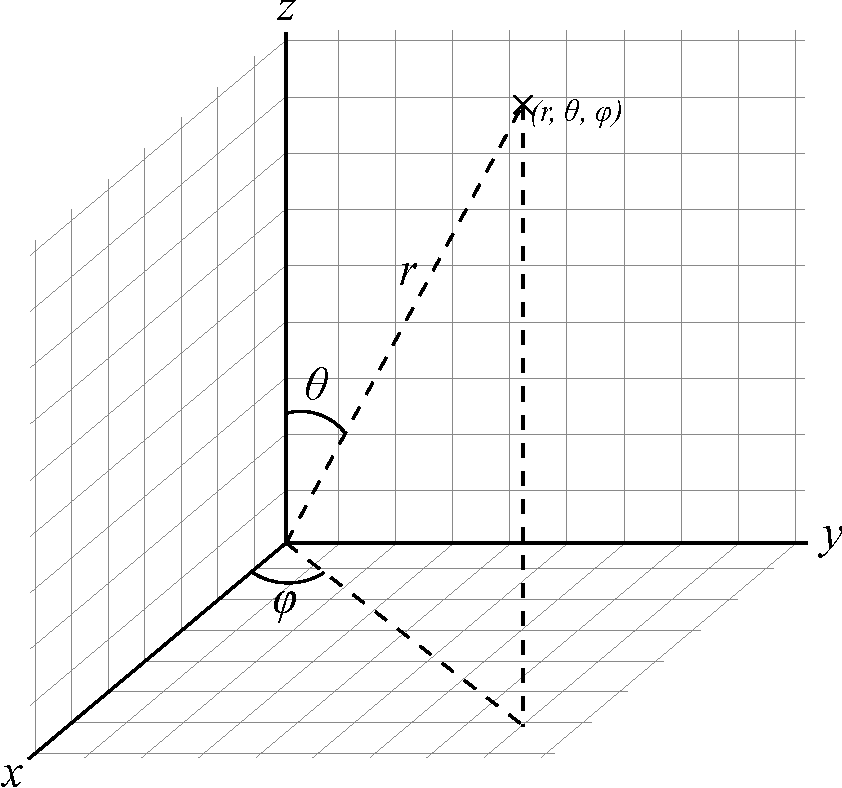
\includegraphics[width=130mm]{../img/spherical}
  \caption{Sférická soustava souřadnic \cite{wiki:spherical}}
\end{figure}


\section{Ohnisková vzdálenost a zorný úhel}
 Pro nás nejvýznamější parametr objektivu je ohnisková vzdálenost $f_c$, pomocí které lze určit zorné pole kamery.

\begin{definice}[Ohnisková vzdálenost]\label{def01:3}
  Ohnisková vzdálenost $f_c~\text{[mm]}$ je vzdálenost mezi optickým středem objektivu a rovinou snímače (čipu) při zaostření na nekonečno. \citep{Hosko14}
\end{definice}

Ohnisková vzdálenost se mění, když upravujeme optický zoom. Větší zoom znamená větší ohniskovou vzdálenost a užší zorný úhel. 
My budeme ohniskovou vzdálenost modelovat v pixelech, protože neznáme velikost senzoru webových kamer, ale známe rozlišení jejich snímků.

\begin{lemma}\label{lemma01:1}
  Pro objektiv s ohniskovou vzdáleností $f_c~\text{[px]}$ a snímací čip velilosti $(W, H)~\text{[px]}$ je zorný úhel ve vodorovném směru $\omega_h$ dán vztahem
  \begin{equation}\label{eq01:1}
    \omega_h = 2 \arctan \left(\frac{W}{2f}\right).
  \end{equation}
\end{lemma}
\begin{dukaz}
  Vztah je dán goniometrií pravoúhlého trojúhelníku, jehož odvěsny jsou $f$ a $W/2$.
\end{dukaz}

\begin{figure}[h]\centering
  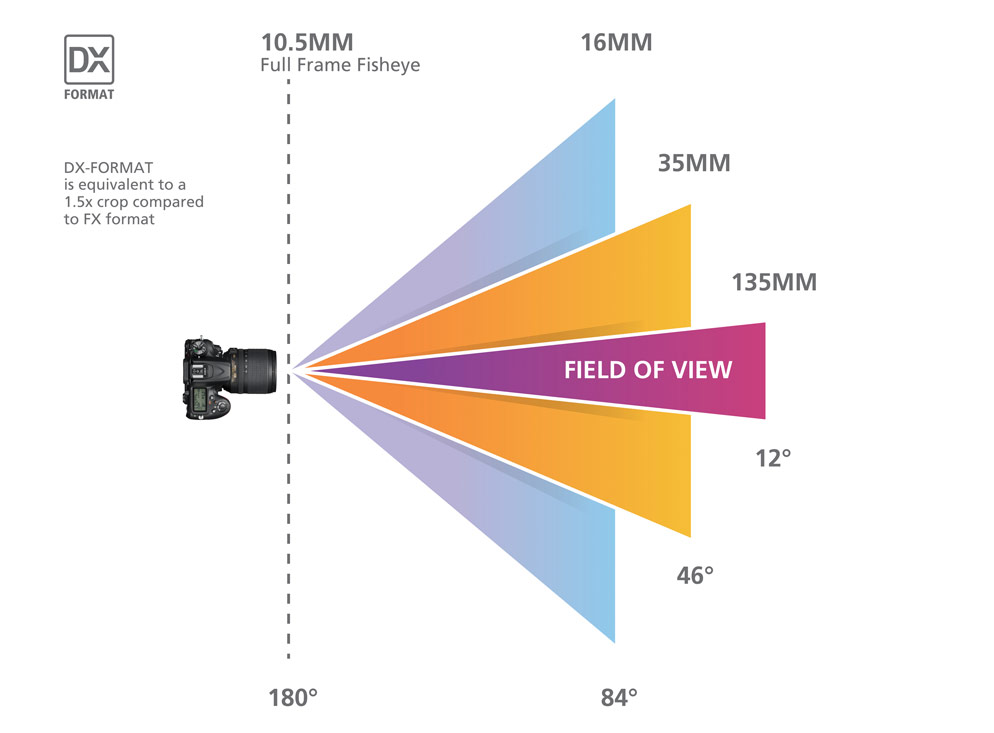
\includegraphics[width=140mm]{../img/fov}
  \caption{Vliv ohniskové vzdálenosti na zorný úhel \cite{nikon}}
\end{figure}


\section{Nalezení bodu na obloze}
Abychom mohli modelovat snímek oblohy kamerou s parametry $(f_c, \theta_c, \phi_c)$, musíme převést pozici pixelu na snímku na pozici bodu na obloze.

\begin{lemma}\label{lemma01:2}(\citealp{Lalonde10}, Appendix B)
  Buď  $\phi_c$ azimut kamery, $\theta_c$ zenit kamery, $f_c~\text{[px]}$ ohnisková vzdálenost kamery, $(W, H)~\text{[px]}$ rozlišení snímku, ($x_p, y_p$) pozice pixelu (horizontální a vertikální vzdálenost od levého horního rohu snímku). Nechť $u_p = x_p - W/2$, $v_p = H/2 - y_p$. Pak
  \begin{equation}\label{eq01:2}
    \theta_p=\arccos \left( \frac{v_p \cdot \sin(\theta_c) + f_c \cdot \cos(\theta_c)}{\sqrt{f_c^2 + u_p^2 + v_p^2}} \right),
  \end{equation}
  \begin{equation}\label{eq01:3}
    \phi_p=\arctan \left( \frac{f_c \cdot \sin(\phi_c) \cdot \sin(\theta_c) - u_p \cdot \cos(\theta_c) - v_p \cdot \sin(\theta_c) \cdot \cos(\phi_c)}{f_c \cdot \cos(\theta_c) \cdot \sin(\phi_c) + u_p \cdot \sin(\theta_c) - v_p \cdot \cos(\theta_c) \cdot \cos(\phi_c)} \right)
  \end{equation}
\end{lemma}
\begin{dukaz}
  Jednotlivé kroky důkazu jsou podrobně popsány v~práci \citet[Appendix B]{Lalonde10}.
\end{dukaz}
  
\begin{lemma}\label{lemma01:3}(\citealp{Lalonde10}, strana 16)
  Nechť $(\phi_c, \theta_c$) je směr kamery, $(\phi_s, \theta_s$) je pozice slunce na obloze, $f_c[px]$ ohnisková vzdálenost kamery, $(W, H)$ rozlišení snímku, ($x_p, y_p$) pozice pixelu (horizontální a vertikální vzdálenost od levého horního rohu snímku). Nechť $u_p = x_p - W/2$, $v_p = H/2 - y_p$. Pak úhel $\gamma_p$ mezi sluncem $(\phi_s, \theta_s$) a bodem na obloze $(\phi_c, \theta_c$) je dán vztahem
  \begin{equation}\label{eq01:4}
    \gamma_p = \arccos \left( \cos(\phi_p) \cdot \cos(\phi_s) + \sin(\phi_p) \cdot \sin(\phi_s) \cdot \cos(\theta_p - \theta_s) \right)
  \end{equation}
\end{lemma}

\begin{figure}[h]\centering
  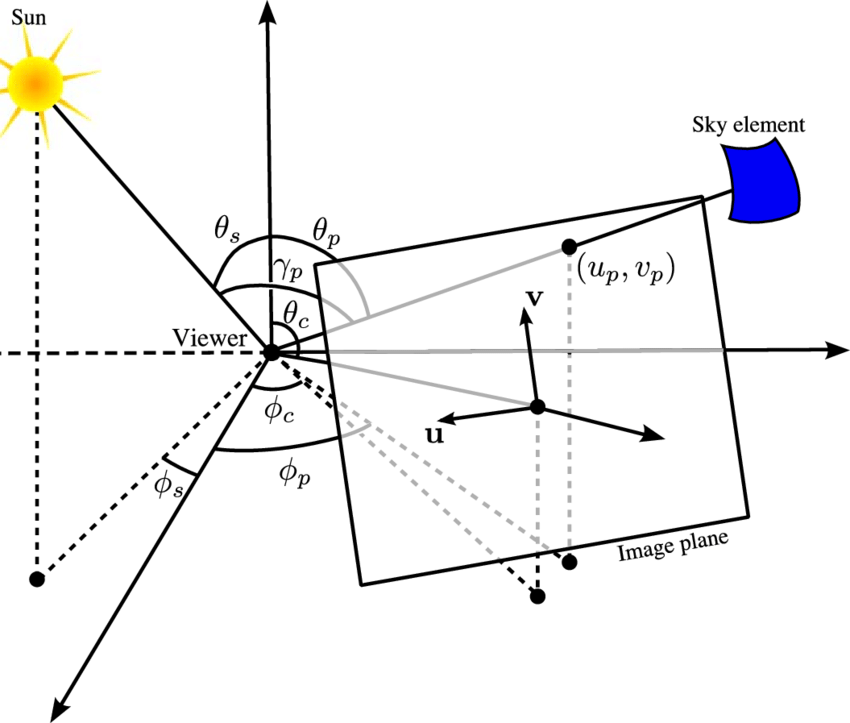
\includegraphics[width=140mm]{../img/uhly}
  \caption{Pozice slunce $(\theta_s, \gamma_s)$, orientace kamery $(\theta_c, \gamma_c)$, pozice bodu na obloze $(\theta_p, \gamma_p)$, úhel bodu na obloze se sluncem $\gamma_p$, pozice bodu na obrázku $(u_p, v_p)$
  (\citealp{Lalonde10}, strana 15)}
\end{figure}

\section{Radiometrie, fotometrie a spektrometrie}
Radiometrie a fotometrie a spektrometrie jsou vědní disciplíny, které se zabývají měřením a analýzou světla a elektromagnetického záření. 
Radiometrie se zaměřuje na kvantitativní měření energie elektromagnetického záření.
Fotometrie se na druhou stranu zaměřuje na měření světla ve vztahu k lidskému vnímání.
Spektrometrie zkoumá vlastnosti světla a elektromagnetického záření v různých vlnových délkách.
Vzhledem k tomu, že lidské oko má různou citlivost na různé vlnové délky světla, fotometrická měření jsou váženy podle vnímání lidského oka. 

Nás nejvíce bude zajímat vztah mezi radiometrickou veličinou zář a fotometrickou veličinou jas.


\begin{definice}[Spektrální odezva]
  Spektrální odezva $V(\lambda)$ je funkce, která popisuje citlivost lidského oka na různé vlnové délky světla.
\end{definice}

\begin{definice}[Spektrální zář a jas]
  Jas $L$ je zář $L_e$ vážená spektrální odezvou lidského oka $V(\lambda)$. Platí:
  \begin{equation}
    L(\lambda) = L_e(\lambda) \cdot V(\lambda)
  \end{equation}
\end{definice}

Příklad využití spektrální citlivosti oka je převod RGB obrázku do jednoho kanálu L \citep{rgbgray}.
\begin{equation}
  L = 0.2126 \cdot R + 0.7152 \cdot G + 0.0722 \cdot B 
\end{equation}

\section{Perezův model oblohy}
Tento analytický model oblohy byl poprvé představen v článku \cite{Perez93}.
Model bere v úvahu zenit pozorovaného bodu $\theta$ a úhel se sluncem $\gamma$.

\begin{veta}\label{veta01:1}\citep{Perez93}
Relativní jas bodu na obloze vůči jasu zenitu je dán vztahem:
\begin{equation}\label{eq01:5}
  l_p = (1 + a \cdot \exp(b/\cos(\theta))) \cdot (1 + c \cdot \exp(d \cdot \gamma) + e \cdot \cos^2(\gamma))
\end{equation}
    Kde ($a, b, c, d, e$) jsou koeficienty modelu, které závisí na meteorologických podmínkách a zeměpisné poloze.
\end{veta}

Výhoda Perezova modelu je jeho jednoduchost. Je vhodný pro simulace, ve kterých se prefetuje výpočetní výkon nad přesností. Jeho nevýhodou je to, že nedokáže zohledňovat více atmosférických vlivů a že jeho parametry $a, b, c, d, e$ je nutné nalézt v tabulkách nebo nastavit pomocí empirických měření.

\section{Pražský model oblohy}

Pražský model oblohy \citep{Prague2021} byl vyvinut na Matematicko-fyzikálni fakultě Univerzity Karlovy. 
Oproti Perezovu modelu nepočítá relativní jas (fotometrická veličina), ale zář (radiometrická veličina). 
Není to analytický model, ale přistupuje k datům vygenerovaným fyzikálním simulátorem Libradtran \citep{Libradtran2016}, které jsou komprimovány do souboru o velikosti cca 2GB. 
Díky tomu je pražský model přesnější a obecnější než Perezův model a zároveň je rychlejší, než fyzikální simulace.

\subsection{Matematický popis}
Pražský model oblohy zohledňuje následující proměnné: 
\begin{itemize}
  \item $\theta_p$: zenit pozorovaného bodu
  \item $\gamma_p$: úhel mezi pozorovaným bodem a sluncem
  \item $\phi_s$: azimut slunce
  \item $\theta_s$: zenit slunce
  \item $viditelnost[km]$ (za jasného dne zhruba 100km)
  \item $albedo$: míra odrazivosti země, v rozsahu od 0 do 1. (Zasněžená krajina má vyšší albedo než travnatá plocha)
  \item vlnová délka [nm]: při generování obrázků nás bude zajímat červená, zelená a modrá barva, které odpovídají vlnovým délkám 650nm, 550nm a 450nm. 
\end{itemize}
a vrací spektrální zář  $L_e [W \cdot sr^{-1} \cdot m^{-2} \cdot nm^{-1}]$.
\subsection{Využití}
Model je použit ve fotorealistickém renderovacím softwaru Corona Renderer od společnosti Chaos Czech a.s. \citep{corona}. 
Jeho hlavní oblasti využití zahrnují architektonické vizualizace, interiérový design, filmový a televizní průmysl, reklamu a 3D vizualizace a animace. Corona Renderer je kompatibilní s programy jako Autodesk 3ds Max a Cinema 4D, což usnadňuje jeho integraci do stávajících pracovních postupů.

\section{Úprava práce}


Práce se tiskne na bílý papír formátu A4. Okraje musí ponechat dost místa na vazbu:
doporučen je horní, dolní a pravý okraj $25\,\rm mm$, levý okraj $40\,\rm mm$.
Číslují se všechny strany kromě obálky a informačních stran na začátku práce;
první číslovaná strana bývá obvykle ta s~obsahem.

Písmo se doporučuje dvanáctibodové ($12\,\rm pt$) se standardní vzdáleností mezi řádky
(pokud píšete ve Wordu nebo podobném programu, odpovídá tomu řádkování $1,5$; v~\TeX{}u
není potřeba nic přepínat). Pro běžný text používejte vzpřímené patkové písmo.
Text matematických vět se obvykle tiskne pro zdůraznění skloněným (slanted) písmem,
není-li k~dispozici, může být zastoupeno kurzívou.

Primárně je doporučován jednostranný tisk (příliš tenkou práci lze obtížně svázat).
Delší práce je lepší tisknout oboustranně a přizpůsobit tomu velikosti okrajů:
$40\,\rm mm$ má vždy \emph{vnitřní} okraj. Rub titulního listu zůstává nepotištěný.

Zkratky použité v textu musí být vysvětleny vždy u prvního výskytu zkratky (v~závorce nebo
v poznámce pod čarou, jde-li o složitější vysvětlení pojmu či zkratky). Pokud je zkratek
více, připojuje se seznam použitých zkratek, včetně jejich vysvětlení a/nebo odkazů
na definici.

Delší převzatý text jiného autora je nutné vymezit uvozovkami nebo jinak vyznačit a řádně
citovat.

\section{Jednoduché příklady}

Čísla v~českém textu obvykle sázíme v~matematickém režimu s~desetinnou čárkou:
%%% Bez \usepackage{icomma}:
% $\pi \doteq 3{,}141\,592\,653\,589$.
%%% S \usepackage{icomma}:
$\pi \doteq 3,141\,592\,653\,589$.
V~matematických textech se považuje za přípustné používat desetinnou tečku
(pro lepší odlišení od čárky v~roli oddělovače). Numerické výsledky se uvádějí
s~přiměřeným počtem desetinných míst.

Mezi číslo a jednotku patří úzká mezera: šířka stránky A4 činí $210\,\rm mm$, což si
pamatuje pouze $5\,\%$ autorů. Pokud ale údaj slouží jako přívlastek, mezeru vynecháváme:
$25\rm mm$ okraj, $95\%$ interval spolehlivosti.

Rozlišujeme různé druhy pomlček:
červeno-černý (krátká pomlčka),
strana 16--22 (střední),
$45-44$ (matematické minus),
a~toto je --- jak se asi dalo čekat --- vložená věta ohraničená dlouhými pomlčkami.

V~českém textu se používají \uv{české} uvozovky, nikoliv ``anglické''.

% V tomto odstavci se vlnka zviditelňuje
{
\def~{{\tt\char126}}
Na některých místech je potřeba zabránit lámání řádku (v~\TeX{}u značíme vlnovkou):
u~předložek (neslabičnych, nebo obecně jednopísmenných), vrchol~$v$, před $k$~kroky,
a~proto, \dots{} obecně kdekoliv, kde by při rozlomení čtenář \uv{ško\-brt\-nul}.
}

\section{Matematické vzorce a výrazy}

Proměnné sázíme kurzívou (to \TeX{} v~matematickém módu dělá sám, ale
nezapomínejte na to v~okolním textu a také si matematický mód zapněte).
Názvy funkcí sázíme vzpřímeně. Tedy například:
$\var(X) = \E X^2 - \bigl(\E X \bigr)^2$.

Zlomky uvnitř odstavce (třeba $\frac{5}{7}$ nebo $\frac{x+y}{2}$) mohou
být příliš stísněné, takže je lepší sázet jednoduché zlomky s~lomítkem:
$5/7$, $(x+y)/2$.

Nechť
\[   % LaTeXová náhrada klasického TeXového $$
  \mathbb{X} = \begin{pmatrix}
    \T{\bm x_1} \\
    \vdots      \\
    \T{\bm x_n}
  \end{pmatrix}.
\]
Povšimněme si tečky za~maticí. Byť je matematický text vysázen
ve~specifickém prostředí, stále je gramaticky součástí věty a~tudíž je
zapotřebí neopomenout patřičná interpunkční znaménka. Výrazy, na které
chceme později odkazovat, je vhodné očíslovat:
\begin{equation}\label{eq01:Xmat}
  \mathbb{X} = \begin{pmatrix}
    \T{\bm x_1} \\
    \vdots      \\
    \T{\bm x_n}
  \end{pmatrix}.
\end{equation}
Výraz \eqref{eq01:Xmat} definuje matici $\mathbb{X}$. Pro lepší čitelnost
a~přehlednost textu je vhodné číslovat pouze ty výrazy, na které se
autor někde v~další části textu odkazuje. To jest, nečíslujte
automaticky všechny výrazy vysázené některým z~matematických
prostředí.

Zarovnání vzorců do několika sloupečků:
\begin{alignat*}{3}
  S(t) & = \pr(T > t),    & \qquad t & >0 & \qquad & \text{ (zprava spojitá),} \\
  F(t) & = \pr(T \leq t), & \qquad t & >0 & \qquad & \text{ (zprava spojitá).}
\end{alignat*}

Dva vzorce se spojovníkem:
\begin{equation}\label{eq01:FS}
  \left.
  \begin{aligned}
    S(t) & = \pr(T > t)    \\[1ex]
    F(t) & = \pr(T \leq t)
  \end{aligned}
  \;	% zde pomůže ručně vynechat trochu místa
  \right\}
  \quad t>0 \qquad \text{(zprava spojité).}
\end{equation}

Dva centrované nečíslované vzorce:
\begin{gather*}
  \bm Y = \mathbb{X}\bm\beta + \bm\varepsilon, \\[1ex]
  \mathbb{X} = \begin{pmatrix} 1 & \T{\bm x_1} \\ \vdots & \vdots \\ 1 &
                \T{\bm x_n}\end{pmatrix}.
\end{gather*}
Dva centrované číslované vzorce:
\begin{gather}
  \bm Y = \mathbb{X}\bm\beta + \bm\varepsilon, \label{eq02:Y}\\[1ex]
  \mathbb{X} = \begin{pmatrix} 1 & \T{\bm x_1} \label{eq03:X} \\ \vdots & \vdots \\ 1 &
                \T{\bm x_n}\end{pmatrix}.
\end{gather}

Definice rozdělená na dva případy:
\[
  P_{r-j}=
  \begin{cases}
    0,                  & \text{je-li $r-j$ liché}, \\
    r!\,(-1)^{(r-j)/2}, & \text{je-li $r-j$ sudé}.
  \end{cases}
\]
Všimněte si použití interpunkce v této konstrukci. Čárky a tečky se
dávají na místa, kam podle jazykových pravidel patří.

\begin{align}
  x & = y_1-y_2+y_3-y_5+y_8-\dots = &  & \text{z \eqref{eq02:Y}} \nonumber     \\
    & = y'\circ y^* =               &  & \text{podle \eqref{eq03:X}} \nonumber \\
    & = y(0) y'                     &  & \text {z Axiomu 1.}
\end{align}


Dva zarovnané vzorce nečíslované:
\begin{align*}
  L(\bm\theta)    & = \prod_{i=1}^n f_i(y_i;\,\bm\theta), \\
  \ell(\bm\theta) & = \log\bigl\{L(\bm\theta)\bigr\} =
  \sum_{i=1}^n \log\bigl\{f_i(y_i;\,\bm\theta)\bigr\}.
\end{align*}
Dva zarovnané vzorce, první číslovaný:
\begin{align}
  L(\bm\theta)    & = \prod_{i=1}^n f_i(y_i;\,\bm\theta), \label{eq01:L} \\
  \ell(\bm\theta) & = \log\bigl\{L(\bm\theta)\bigr\} =
  \sum_{i=1}^n \log\bigl\{f_i(y_i;\,\bm\theta)\bigr\}. \nonumber
\end{align}

Vzorec na dva řádky, první řádek zarovnaný vlevo, druhý vpravo, nečíslovaný:
\begin{multline*}
  \ell(\mu,\,\sigma^2) = \log\bigl\{L(\mu,\,\sigma^2)\bigr\} =
  \sum_{i=1}^n \log\bigl\{f_i(y_i;\,\mu,\,\sigma^2)\bigr\}= \\
  = -\,\frac{n}{2}\,\log(2\pi\sigma^2) \,-\,
  \frac{1}{2\sigma^2}\sum_{i=1}^n\,(y_i - \mu)^2.
\end{multline*}

Vzorec na dva řádky, zarovnaný na $=$, číslovaný uprostřed:
\begin{equation}\label{eq01:ell}
  \begin{split}
    \ell(\mu,\,\sigma^2) &= \log\bigl\{L(\mu,\,\sigma^2)\bigr\} =
    \sum_{i=1}^n \log\bigl\{f(y_i;\,\mu,\,\sigma^2)\bigr\}= \\
    & = -\,\frac{n}{2}\,\log(2\pi\sigma^2) \,-\,
    \frac{1}{2\sigma^2}\sum_{i=1}^n\,(y_i - \mu)^2.
  \end{split}
\end{equation}

\section{Definice, věty, důkazy, \dots}

Konstrukce typu definice, věta, důkaz, příklad, \dots je vhodné
odlišit od okolního textu a~případně též číslovat s~možností použití
křížových odkazů. Pro každý typ těchto konstrukcí je vhodné mít
v~souboru s~makry (\texttt{makra.tex}) nadefinované jedno prostředí,
které zajistí jak vizuální odlišení od okolního textu, tak
automatické číslování s~možností křížově odkazovat.

\begin{definice}
  Nechť náhodné veličiny $X_1,\dots,X_n$ jsou definovány na témž
  prav\-dě\-po\-dob\-nost\-ním prostoru $(\omega,\,\mathcal{A},\,\pr)$. Pak
  vektor $\bm X = \T{(X_1,\dots,X_n)}$ nazveme \emph{náhodným
    vektorem}.
\end{definice}

\begin{definice}[náhodný vektor]
  Nechť náhodné veličiny $X_1,\dots,X_n$ jsou definovány na témž
  pravděpodobnostním prostoru $(\omega,\,\mathcal{A},\,\pr)$. Pak
  vektor $\bm X = \T{(X_1,\dots,X_n)}$ nazveme \emph{náhodným
    vektorem}.
\end{definice}
Definice~\ref{def01:1} ukazuje použití prostředí pro sazbu definice
bez titulku, definice~\ref{def01:2} ukazuje použití prostředí pro
sazbu definice s~titulkem.

\begin{veta}\label{veta01:1}
  Náhodný vektor $\bm X$ je měřitelné zobrazení prostoru
  $(\omega,\,\mathcal{A},\,\pr)$ do $(\R_n,\,\mathcal{B}_n)$.
\end{veta}

\begin{lemma}[\citealp{Andel07}, str. 29]
  Náhodný vektor $\bm X$ je měřitelné zobrazení prostoru
  $(\omega,\,\mathcal{A},\,\pr)$ do $(\R_n,\,\mathcal{B}_n)$.
\end{lemma}
\begin{dukaz}
  Jednotlivé kroky důkazu jsou podrobně popsány v~práci \citet[str.
    29]{Andel07}.
\end{dukaz}
Věta~\ref{veta01:1} ukazuje použití prostředí pro sazbu matematické
věty bez titulku, lemma~\ref{veta01:2} ukazuje použití prostředí pro
sazbu matematické věty s~titulkem. Lemmata byla zavedena v~hlavním
souboru tak, že sdílejí číslování s~větami.
